% Created by tikzDevice version 0.12.3.1 on 2021-12-17 00:23:02
% !TEX encoding = UTF-8 Unicode
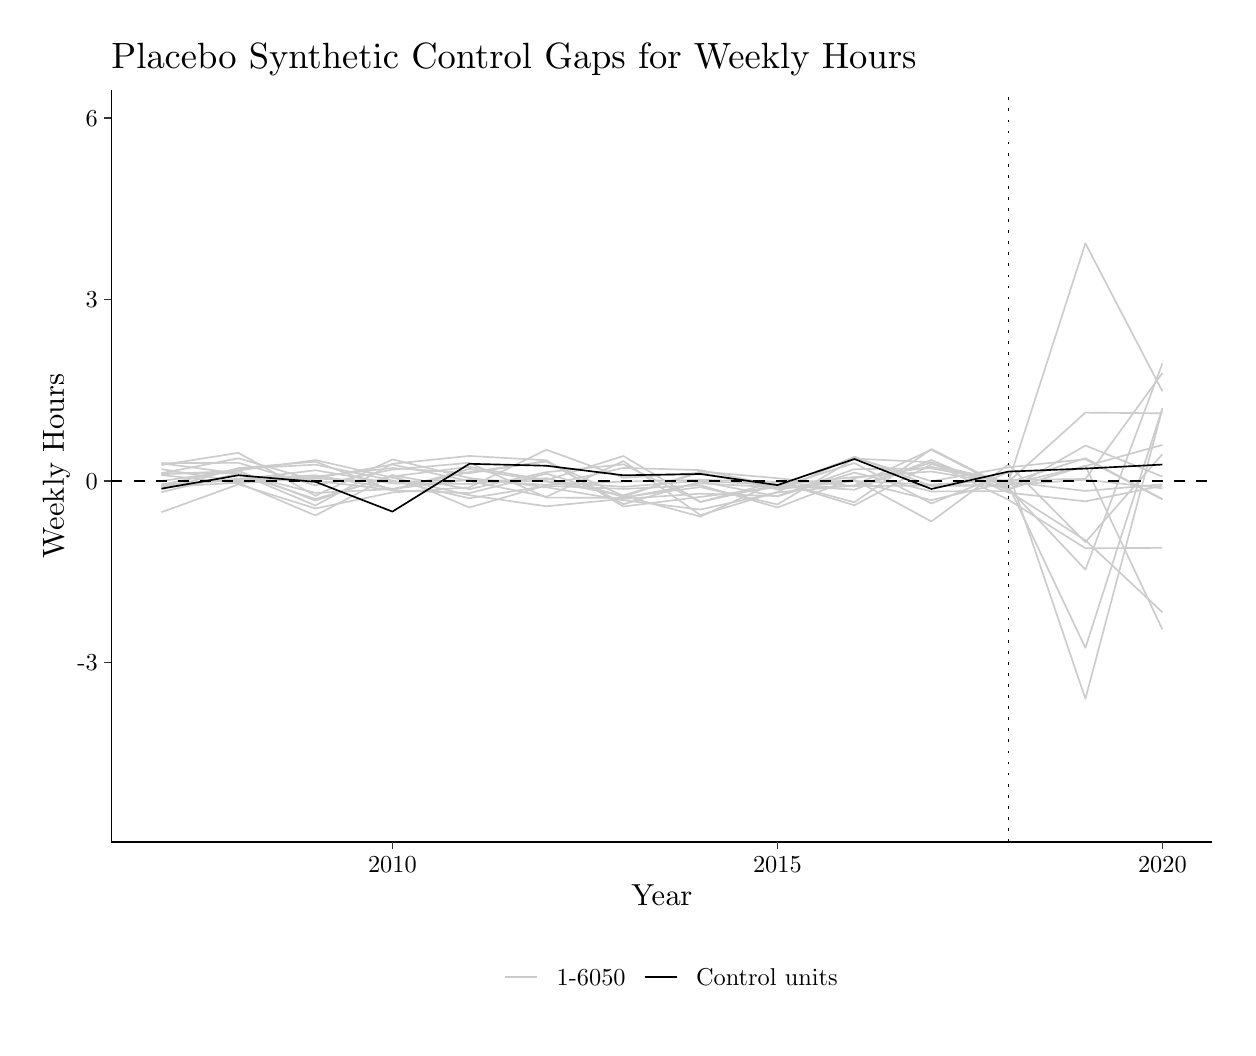
\begin{tikzpicture}[x=1pt,y=1pt]
\definecolor{fillColor}{RGB}{255,255,255}
\path[use as bounding box,fill=fillColor,fill opacity=0.00] (0,0) rectangle (433.62,361.35);
\begin{scope}
\path[clip] (  0.00,  0.00) rectangle (433.62,361.35);
\definecolor{drawColor}{RGB}{255,255,255}
\definecolor{fillColor}{RGB}{255,255,255}

\path[draw=drawColor,line width= 0.6pt,line join=round,line cap=round,fill=fillColor] (  0.00,  0.00) rectangle (433.62,361.35);
\end{scope}
\begin{scope}
\path[clip] ( 30.25, 67.14) rectangle (428.12,338.69);
\definecolor{drawColor}{gray}{0.80}

\path[draw=drawColor,line width= 0.6pt,line join=round] ( 48.33,195.41) --
	( 76.15,196.88) --
	(103.98,185.08) --
	(131.80,199.63) --
	(159.62,187.97) --
	(187.45,196.00) --
	(215.27,202.27) --
	(243.09,201.47) --
	(270.92,195.79) --
	(298.74,206.02) --
	(326.56,197.46) --
	(354.39,202.48) --
	(382.21,205.42) --
	(410.03,190.89);

\path[draw=drawColor,line width= 0.6pt,line join=round] ( 48.33,197.56) --
	( 76.15,201.34) --
	(103.98,205.10) --
	(131.80,198.75) --
	(159.62,192.40) --
	(187.45,188.40) --
	(215.27,191.09) --
	(243.09,192.96) --
	(270.92,192.08) --
	(298.74,201.82) --
	(326.56,202.10) --
	(354.39,197.04) --
	(382.21,205.77) --
	(410.03,190.98);

\path[draw=drawColor,line width= 0.6pt,line join=round] ( 48.33,200.36) --
	( 76.15,205.73) --
	(103.98,197.66) --
	(131.80,194.23) --
	(159.62,201.91) --
	(187.45,197.36) --
	(215.27,192.38) --
	(243.09,200.54) --
	(270.92,194.55) --
	(298.74,197.51) --
	(326.56,190.61) --
	(354.39,197.26) --
	(382.21,193.93) --
	(410.03,196.33);

\path[draw=drawColor,line width= 0.6pt,line join=round] ( 48.33,195.77) --
	( 76.15,198.06) --
	(103.98,201.42) --
	(131.80,196.67) --
	(159.62,196.48) --
	(187.45,198.56) --
	(215.27,191.96) --
	(243.09,200.99) --
	(270.92,198.55) --
	(298.74,195.68) --
	(326.56,195.89) --
	(354.39,196.13) --
	(382.21,198.00) --
	(410.03,194.92);

\path[draw=drawColor,line width= 0.6pt,line join=round] ( 48.33,203.92) --
	( 76.15,200.21) --
	(103.98,193.24) --
	(131.80,194.60) --
	(159.62,200.77) --
	(187.45,204.56) --
	(215.27,192.16) --
	(243.09,184.67) --
	(270.92,197.25) --
	(298.74,188.76) --
	(326.56,203.58) --
	(354.39,197.16) --
	(382.21,283.42) --
	(410.03,229.95);

\path[draw=drawColor,line width= 0.6pt,line join=round] ( 48.33,186.26) --
	( 76.15,196.33) --
	(103.98,187.62) --
	(131.80,193.41) --
	(159.62,195.25) --
	(187.45,208.83) --
	(215.27,198.73) --
	(243.09,200.43) --
	(270.92,195.16) --
	(298.74,204.02) --
	(326.56,189.40) --
	(354.39,200.76) --
	(382.21,118.84) --
	(410.03,223.63);

\path[draw=drawColor,line width= 0.6pt,line join=round] ( 48.33,203.31) --
	( 76.15,207.71) --
	(103.98,192.19) --
	(131.80,205.34) --
	(159.62,198.61) --
	(187.45,195.28) --
	(215.27,190.58) --
	(243.09,187.22) --
	(270.92,193.41) --
	(298.74,196.00) --
	(326.56,208.83) --
	(354.39,194.55) --
	(382.21,203.02) --
	(410.03,143.87);

\path[draw=drawColor,line width= 0.6pt,line join=round] ( 48.33,195.63) --
	( 76.15,198.39) --
	(103.98,199.59) --
	(131.80,194.72) --
	(159.62,197.97) --
	(187.45,197.36) --
	(215.27,195.43) --
	(243.09,197.62) --
	(270.92,195.99) --
	(298.74,198.96) --
	(326.56,200.96) --
	(354.39,196.34) --
	(382.21,202.90) --
	(410.03,210.56);

\path[draw=drawColor,line width= 0.6pt,line join=round] ( 48.33,200.33) --
	( 76.15,200.36) --
	(103.98,188.67) --
	(131.80,203.76) --
	(159.62,206.59) --
	(187.45,205.03) --
	(215.27,188.31) --
	(243.09,191.80) --
	(270.92,195.29) --
	(298.74,195.62) --
	(326.56,204.20) --
	(354.39,190.76) --
	(382.21,173.22) --
	(410.03,173.38);

\path[draw=drawColor,line width= 0.6pt,line join=round] ( 48.33,196.34) --
	( 76.15,197.91) --
	(103.98,198.43) --
	(131.80,197.26) --
	(159.62,197.85) --
	(187.45,196.16) --
	(215.27,197.32) --
	(243.09,197.98) --
	(270.92,197.24) --
	(298.74,197.50) --
	(326.56,196.28) --
	(354.39,197.89) --
	(382.21,198.28) --
	(410.03,236.56);

\path[draw=drawColor,line width= 0.6pt,line join=round] ( 48.33,196.18) --
	( 76.15,201.96) --
	(103.98,203.44) --
	(131.80,197.74) --
	(159.62,191.28) --
	(187.45,195.79) --
	(215.27,194.67) --
	(243.09,195.98) --
	(270.92,187.96) --
	(298.74,198.57) --
	(326.56,202.62) --
	(354.39,197.23) --
	(382.21,222.24) --
	(410.03,222.01);

\path[draw=drawColor,line width= 0.6pt,line join=round] ( 48.33,193.48) --
	( 76.15,200.25) --
	(103.98,191.02) --
	(131.80,199.19) --
	(159.62,202.65) --
	(187.45,197.84) --
	(215.27,206.56) --
	(243.09,189.98) --
	(270.92,197.30) --
	(298.74,189.85) --
	(326.56,209.08) --
	(354.39,195.01) --
	(382.21,165.50) --
	(410.03,240.05);

\path[draw=drawColor,line width= 0.6pt,line join=round] ( 48.33,203.98) --
	( 76.15,204.10) --
	(103.98,195.98) --
	(131.80,201.67) --
	(159.62,204.11) --
	(187.45,191.55) --
	(215.27,191.41) --
	(243.09,196.71) --
	(270.92,195.22) --
	(298.74,197.99) --
	(326.56,182.92) --
	(354.39,203.50) --
	(382.21,175.44) --
	(410.03,207.22);

\path[draw=drawColor,line width= 0.6pt,line join=round] ( 48.33,199.68) --
	( 76.15,196.75) --
	(103.98,198.56) --
	(131.80,203.50) --
	(159.62,197.49) --
	(187.45,191.84) --
	(215.27,204.72) --
	(243.09,185.21) --
	(270.92,193.59) --
	(298.74,206.33) --
	(326.56,195.70) --
	(354.39,196.01) --
	(382.21,137.25) --
	(410.03,223.84);

\path[draw=drawColor,line width= 0.6pt,line join=round] ( 48.33,201.82) --
	( 76.15,197.29) --
	(103.98,199.11) --
	(131.80,202.22) --
	(159.62,200.36) --
	(187.45,204.77) --
	(215.27,189.13) --
	(243.09,197.35) --
	(270.92,191.94) --
	(298.74,200.56) --
	(326.56,193.76) --
	(354.39,193.91) --
	(382.21,176.10) --
	(410.03,150.11);

\path[draw=drawColor,line width= 0.6pt,line join=round] ( 48.33,199.96) --
	( 76.15,201.21) --
	(103.98,190.45) --
	(131.80,199.66) --
	(159.62,194.60) --
	(187.45,200.74) --
	(215.27,203.56) --
	(243.09,189.97) --
	(270.92,196.15) --
	(298.74,194.39) --
	(326.56,205.12) --
	(354.39,193.35) --
	(382.21,190.18) --
	(410.03,195.83);

\path[draw=drawColor,line width= 0.6pt,line join=round] ( 48.33,194.42) --
	( 76.15,202.22) --
	(103.98,204.52) --
	(131.80,194.16) --
	(159.62,193.15) --
	(187.45,200.19) --
	(215.27,191.74) --
	(243.09,195.33) --
	(270.92,189.07) --
	(298.74,205.63) --
	(326.56,204.31) --
	(354.39,194.33) --
	(382.21,210.36) --
	(410.03,199.13);
\definecolor{drawColor}{RGB}{0,0,0}

\path[draw=drawColor,line width= 0.6pt,dash pattern=on 1pt off 3pt ,line join=round] (354.39, 67.14) -- (354.39,338.69);

\path[draw=drawColor,line width= 0.6pt,dash pattern=on 4pt off 4pt ,line join=round] ( 30.25,197.55) -- (428.12,197.55);

\path[draw=drawColor,line width= 0.6pt,line join=round] ( 48.33,194.78) --
	( 76.15,199.60) --
	(103.98,197.25) --
	(131.80,186.48) --
	(159.62,203.75) --
	(187.45,203.05) --
	(215.27,199.60) --
	(243.09,200.07) --
	(270.92,196.05) --
	(298.74,205.48) --
	(326.56,194.65) --
	(354.39,200.94) --
	(382.21,202.03) --
	(410.03,203.48);
\end{scope}
\begin{scope}
\path[clip] (  0.00,  0.00) rectangle (433.62,361.35);
\definecolor{drawColor}{RGB}{0,0,0}

\path[draw=drawColor,line width= 0.6pt,line join=round] ( 30.25, 67.14) --
	( 30.25,338.69);
\end{scope}
\begin{scope}
\path[clip] (  0.00,  0.00) rectangle (433.62,361.35);
\definecolor{drawColor}{RGB}{0,0,0}

\node[text=drawColor,anchor=base east,inner sep=0pt, outer sep=0pt, scale=  0.88] at ( 25.30,128.98) {-3};

\node[text=drawColor,anchor=base east,inner sep=0pt, outer sep=0pt, scale=  0.88] at ( 25.30,194.52) {0};

\node[text=drawColor,anchor=base east,inner sep=0pt, outer sep=0pt, scale=  0.88] at ( 25.30,260.06) {3};

\node[text=drawColor,anchor=base east,inner sep=0pt, outer sep=0pt, scale=  0.88] at ( 25.30,325.59) {6};
\end{scope}
\begin{scope}
\path[clip] (  0.00,  0.00) rectangle (433.62,361.35);
\definecolor{drawColor}{gray}{0.20}

\path[draw=drawColor,line width= 0.6pt,line join=round] ( 27.50,132.01) --
	( 30.25,132.01);

\path[draw=drawColor,line width= 0.6pt,line join=round] ( 27.50,197.55) --
	( 30.25,197.55);

\path[draw=drawColor,line width= 0.6pt,line join=round] ( 27.50,263.09) --
	( 30.25,263.09);

\path[draw=drawColor,line width= 0.6pt,line join=round] ( 27.50,328.63) --
	( 30.25,328.63);
\end{scope}
\begin{scope}
\path[clip] (  0.00,  0.00) rectangle (433.62,361.35);
\definecolor{drawColor}{RGB}{0,0,0}

\path[draw=drawColor,line width= 0.6pt,line join=round] ( 30.25, 67.14) --
	(428.12, 67.14);
\end{scope}
\begin{scope}
\path[clip] (  0.00,  0.00) rectangle (433.62,361.35);
\definecolor{drawColor}{gray}{0.20}

\path[draw=drawColor,line width= 0.6pt,line join=round] (131.80, 64.39) --
	(131.80, 67.14);

\path[draw=drawColor,line width= 0.6pt,line join=round] (270.92, 64.39) --
	(270.92, 67.14);

\path[draw=drawColor,line width= 0.6pt,line join=round] (410.03, 64.39) --
	(410.03, 67.14);
\end{scope}
\begin{scope}
\path[clip] (  0.00,  0.00) rectangle (433.62,361.35);
\definecolor{drawColor}{RGB}{0,0,0}

\node[text=drawColor,anchor=base,inner sep=0pt, outer sep=0pt, scale=  0.88] at (131.80, 56.13) {2010};

\node[text=drawColor,anchor=base,inner sep=0pt, outer sep=0pt, scale=  0.88] at (270.92, 56.13) {2015};

\node[text=drawColor,anchor=base,inner sep=0pt, outer sep=0pt, scale=  0.88] at (410.03, 56.13) {2020};
\end{scope}
\begin{scope}
\path[clip] (  0.00,  0.00) rectangle (433.62,361.35);
\definecolor{drawColor}{RGB}{0,0,0}

\node[text=drawColor,anchor=base,inner sep=0pt, outer sep=0pt, scale=  1.10] at (229.18, 44.09) {Year};
\end{scope}
\begin{scope}
\path[clip] (  0.00,  0.00) rectangle (433.62,361.35);
\definecolor{drawColor}{RGB}{0,0,0}

\node[text=drawColor,rotate= 90.00,anchor=base,inner sep=0pt, outer sep=0pt, scale=  1.10] at ( 13.08,202.92) {Weekly Hours};
\end{scope}
\begin{scope}
\path[clip] (  0.00,  0.00) rectangle (433.62,361.35);
\definecolor{fillColor}{RGB}{255,255,255}

\path[fill=fillColor] (160.19,  5.50) rectangle (298.18, 30.95);
\end{scope}
\begin{scope}
\path[clip] (  0.00,  0.00) rectangle (433.62,361.35);
\definecolor{drawColor}{gray}{0.80}

\path[draw=drawColor,line width= 0.6pt,line join=round] (172.64, 18.23) -- (184.20, 18.23);
\end{scope}
\begin{scope}
\path[clip] (  0.00,  0.00) rectangle (433.62,361.35);
\definecolor{drawColor}{gray}{0.80}

\path[draw=drawColor,line width= 0.6pt,line join=round] (172.64, 18.23) -- (184.20, 18.23);
\end{scope}
\begin{scope}
\path[clip] (  0.00,  0.00) rectangle (433.62,361.35);
\definecolor{drawColor}{RGB}{0,0,0}

\path[draw=drawColor,line width= 0.6pt,line join=round] (223.02, 18.23) -- (234.58, 18.23);
\end{scope}
\begin{scope}
\path[clip] (  0.00,  0.00) rectangle (433.62,361.35);
\definecolor{drawColor}{RGB}{0,0,0}

\path[draw=drawColor,line width= 0.6pt,line join=round] (223.02, 18.23) -- (234.58, 18.23);
\end{scope}
\begin{scope}
\path[clip] (  0.00,  0.00) rectangle (433.62,361.35);
\definecolor{drawColor}{RGB}{0,0,0}

\node[text=drawColor,anchor=base west,inner sep=0pt, outer sep=0pt, scale=  0.88] at (191.14, 15.20) {1-6050};
\end{scope}
\begin{scope}
\path[clip] (  0.00,  0.00) rectangle (433.62,361.35);
\definecolor{drawColor}{RGB}{0,0,0}

\node[text=drawColor,anchor=base west,inner sep=0pt, outer sep=0pt, scale=  0.88] at (241.53, 15.20) {Control units};
\end{scope}
\begin{scope}
\path[clip] (  0.00,  0.00) rectangle (433.62,361.35);
\definecolor{drawColor}{RGB}{0,0,0}

\node[text=drawColor,anchor=base west,inner sep=0pt, outer sep=0pt, scale=  1.32] at ( 30.25,346.76) {Placebo Synthetic Control Gaps for Weekly Hours};
\end{scope}
\end{tikzpicture}
